The space for the conveyor belts is divided into squares of $1 \times 1$ unit, in which the user can build conveyor belts. The conveyor belts also have size $1 \times 1$, and the user can only put a conveyor belt exactly inside a square. We will call such objects \textit{blocks}. There are several blocks for conveyor belts, for example a block with a horizontal conveyor belt, a block with a sloped conveyor belt and a block with a bend.O

The user can also stack blocks. Every block has an height of $1/2$ unit \textbf{(dat is niet waar, stijgende blokken hebben een hoogte van $1$ unit)}. Blocks can also be rotated by the user, but only in $90\,^\circ$-steps.

If the user places two blocks with the same orientation adjacent to each other, they will be drawn as one long conveyor belt. This also happens when a horizontal block is joined with a sloped block. See Figure~\ref{fig:blocks}.

\begin{figure}
  \begin{center}
    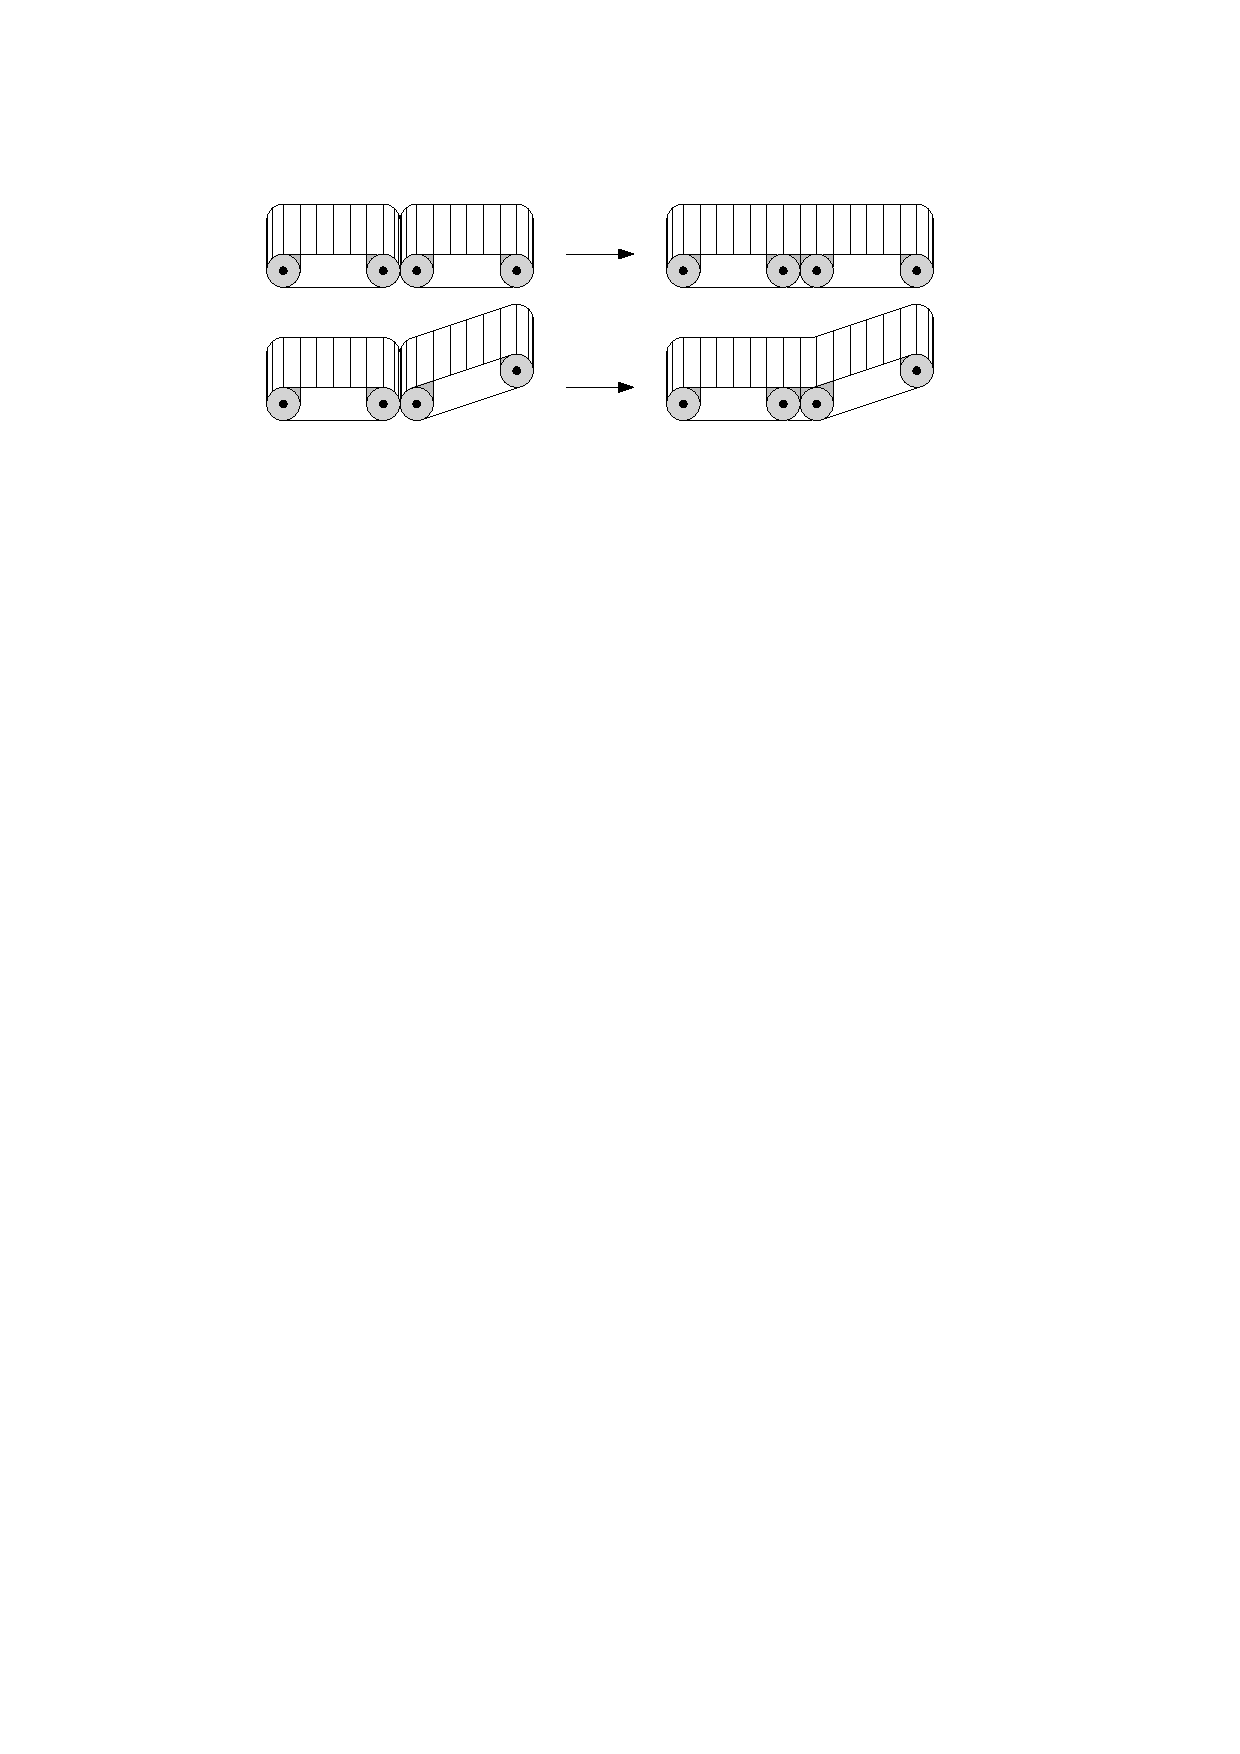
\includegraphics{blocks}
    \caption{Adjacent blocks are drawn as one large conveyor belt.}
    \label{fig:blocks}
  \end{center}
\end{figure}
